\chapter{Introduction}
The Standard Model (SM) in particle physics is the theory that describes the interactions between three fundamental forces, out of the four known  (gravitational, electromagnetic, strong and weak), and the known fundamental particles. The gravitational force is not included in the SM, since the magnitude of its strength is neglectable in comparison with the other three forces.

The  theory was developed throughout the second half of the  20th century by the hard work of physicists around the world, with the current formulation being established in the mid 70s.\\
In high energy physics, precise measurements are the core of any experiment. A key quantity is the luminosity, and its precise determination is an important aspect. The search for low incidence processes whose observation is not yet confirmed, such as the $H\rightarrow\gamma + Z$ channel, relies in the accumulation and precise measurements of luminosity.
\section{The Standard Model}


 The SM classifies all known fundamental particles into two major groups, fermions, particles with spin $1/2$, and bosons, particles responsible for mediating the fundamental forces and integer spin.
Fermions are divided into two families of particles, leptons and quarks. There exist 6 leptons in the SM, first there are charged particles,  electrons ($e$), muons ($\mu$) and the taus ($\tau$) with an electric charge of $-1$ and spin of $1/2$. To each of these particles corresponds a chargeless neutrino, $\nu_{e}$,$\nu_{\mu}$ and $\nu_{\tau}$.

Leptons can be found in nature existing by themselves, and along with quarks, comprise the majority of matter in the universe. Electrons can be found “circling”  atoms, muons can be found raining from the sky due to cosmic rays interacting with particles on the atmosphere and, while taus are a little bit tricky to find due to their short life time ($2.9\times10^{-13}$ s), they do exist by themselves; however, this cannot be said for quarks, since they are only found forming other particles called  hadrons. Hadrons can be a combination of two quarks called mesons, usually a quark-antiquark combination or a combination of three quarks called baryons, an example of a meson would be a pion ($\pi$). Neutrons and protons are made by a combination of three quarks, so they are classified as baryons.
Quarks were first theorised by Murray Gell-Mann and George Zweig in 1964 and later discovered by experiments conducted at the Stanford Linear Accelerator Center (SLAC) in 1968 \cite{griff}. A total of 6 quarks were discovered over a period of 26 years, in order of discovery these are: up ($u$) (1968), down ($d$) (1968), strange ($s$) (1968), charm ($c$) (1974), bottom ($b$) (1977), top ($t$) (1995).

Quarks are the only fermions that interact with all three fundamental forces included in the SM, they possess electric charge, color charge (the strong force equivalent of electric charge), weak charge, mass and spin $ 1/2$ as do all fermions. The $u$, $c$ and $t$ quarks have an electric charge of $2 /3$ and the $d$, $s$ and $b$ quark have an electric charge of $-1/3$. Table \ref{SM table} shows which fermions interact with the different forces. 
%%%%%%%%%%%%%%%%%%%%%%%%%%%%%%%%%%%%%%%%%%%%%%%%%%%%%%%%%%%%%%%%%%%%%%%%%%%%%%%%%%%%%%%%%%%%%%%%%%%%%%%%%%%%%%%%%%%%%%%%%%%%%%%%%%%%%%%%%%%%%%%%%%%%%%%%%%%%%%%%%%%%%%%%%%%%%%%%%%%%%%%%%%%%%%%%%%%%%%%%%%
\begin{table}[H]
\centering
\caption[Fundamental forces and the fermions]{Fundamental forces and the fermions they interact with \cite{Thomson:2013zua}.}
\renewcommand{\arraystretch}{1.5}
\begin{tabular}{|c|c c c|c|c|c|}
\hline 
\multicolumn{2}{|c}{}&  & & Electromagnetic & Strong & Weak\\
\hline
\multirow{2}{*}{Quarks}&u&c&t &\multirow{2}{*}{\checkmark}&\multirow{2}{*}{\checkmark}&\multirow{2}{*}{\checkmark}\\
& d&s&b&&&\\
\hline
\multirow{2}{*}{Fermions}& $e$&$\mu$&$\tau$ &\checkmark& &\checkmark\\
&$\nu_{e}$&$\nu_{\mu}$&$\nu_{\tau}$&&&\checkmark\\
\hline
\end{tabular} 
\label{SM table}
\end{table}
%%%%%%%%%%%%%%%%%%%%%%%%%%%%%%%%%%%%%%%%%%%%%%%%%%%%%%%%%%%%%%%%%%%%%%%%%%%%%%%%%%%%%%%%%%%%%%%%%%%%%%%%%%%%%%%%%%%%%%%%%%%%%%%%%%%%%%%%%%%%%%%%%%%%%%%%%%%%%%%%%%%%%%%%%%%%%%%%%%%%%%%%%%%%%%%%%%%%%%%%%%%%
 For each fermion that exists, there corresponds an antiparticle. Antiparticles have the same properties as their counterparts, with the only distinction being that they possess opposite electric charge. If an antiparticle comes in contact with a particle, let's say a positron (anti-electron) and an electron, they would annihilate each other.

The SM also comprises particles with integer spin  such as the bosons. Bosons are force carrier particles in charge of mediating the interactions between particles, let's take  classical electromagnetism as an example. Classically, the electrostatic force is described by a scalar field and while this is sufficient for classical electromagnetism, it is fundamentally wrong for quantum dynamics. This would mean that two charged particles interact with each other at a distance, without contact of any kind \cite{Thomson:2013zua}.

In  particle physics, each fundamental force is described by a quantum field theory (QFT) and the interaction between two particles are mediated by gauge boson, a spin-1 particle.  For example,  the electromagnetic force is described by Quantum Electrodynamics (QED)  and mediated by the photon, a  particle with no charge or mass. The strong force is described by Quantum Chromodynamics (QCD) and mediated by a gluon, which has no mass or electric charge, gluons are what bind quarks together to form hadron and like quarks, are only found in these bind states. Finally the weak force is mediated by the $Z$ and $W^{\pm}$ bosons, massive particles with 0 an $\pm 1$ electric charge respectively
\cite{Thomson:2013zua}.\\
The Higgs boson is the last member of the SM, unlike the gauge bosons, the Higgs has spin-0 and is the only fundamental scalar discovered. Figure \ref{sm1} shows all the particles included in the SM.


\begin{center}
  \begin{figure}[ht]
    \centering
    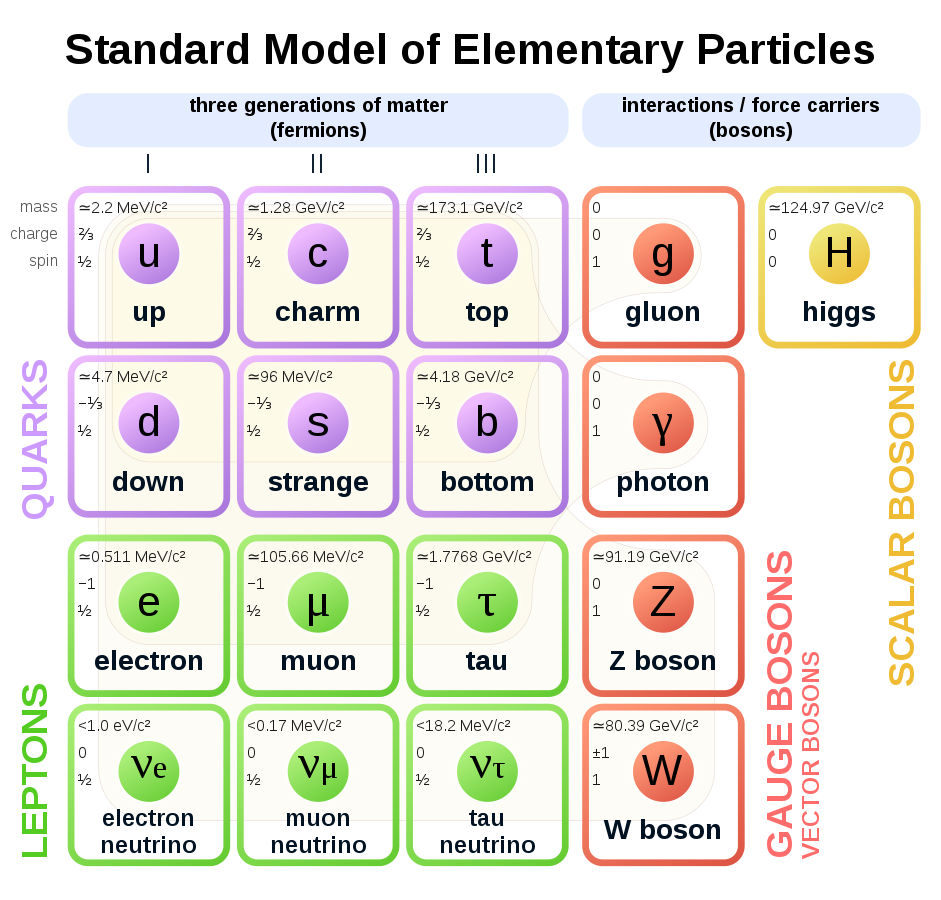
\includegraphics[scale=0.3]{Chapter1/sm1.png}
    \caption[ Standard model of particles]{Particles that compose the standard model and their properties \cite{smtable}.}
    \label{sm1}
  \end{figure}
\end{center}

\section{The Higgs Boson }
The Higgs boson is the latest member of the SM, first theorised in 1964 by Peter Higgs, Robert Brout, François Englert, Gerald Guralnik, C. Richard Hagen and Tom Kibble and later discovered by the ATLAS and CMS experiments at the Large Hadron Collider (LHC) in Geneva Switzerland in 2012. The experiment consisted in proton-proton collisions with a center of mass energy of 7 and 8 TeV, the data analysed from the experiment corresponds to five decay channels: $\gamma\gamma$, $ZZ$, $W^{\pm}W^{\pm}$, $\tau^+\tau^-$ and $b\bar{b}$. With the discovery being made in the  $\gamma\gamma$ and $ZZ$ channels
\cite{higgsd}\cite{Aad_2012}.
The Higgs plays a vital role in the SM, it is responsible for the mechanism that gives every particle their mass. It has a mass of $125.78\pm 0.26$ GeV \cite{CMS:2019drq}, consistent with SM predictions, it does not possess electric or color charge and it is the only fundamental scalar and spin-0 boson.\\
 The discovery of the Higgs is one of the greatest accomplishments of the SM, it shows the hard work that has gone in to developing the theories that compose it \cite{Thomson:2013zua}.


\section{Particle colliders and
detectors}
The discovery of the Higgs marked an important milestone in particle physics, however, this feat required the construction of the LHC, the largest and most powerful particle collider in the world. Particle colliders are the devices where particle physics experiments are conducted. As their name suggests, colliders propel bunches of particles like electrons, protons, positrons, etc. using powerful electromagnetic/electrostatic fields, and make them collide with a fixed target or other particles. These collisions produce other particles that are measured by particle detectors in the site of the collision, this is the means by which new particles are discovered.

Particle colliders come in two types: linear  and circular. Linear colliders  use changing electromagnetic fields to accelerate particles along a straight beam path and make them collide with a fixed target, where particle detectors are located, an example of the linear accelerator would be the Stanford Linear Accelerator Center. While circular colliders to accelerate bunches of particles  in opposite directions in a circular beam fashion, making them collide at key points around the accelerator where particle detectors are located.  The LHC is an example of a circular collider.

The majority of modern experiments in particle physics are conducted in circular colliders, since these are the only ones that can provide the center of mass energy needed to produce heavier particles, like the Higgs or the Top quark. Due to the high energy requirements, circular accelerators are very complex machines composed of many parts, but for the sake of this work, we will only focus on the particle detectors. Modern particle detectors are composed of many layers of subdetectors tasked with measuring the effects that particles have on them, when they pass through. For example, a subdetector may measure the number of hits, tracks or pixel clusters activated during a collision.

The layout of the detector will change to best accommodate the experiments being performed, but in general, these subdetectors can be classified into three categories: Tracking devices, to track the path of a particle; calorimeters, they measure the energy deposited by a particle when it hits and particle identifiers, that use various techniques and the measurements from other subdetectors, to identify the different particles produced in a collision \cite{detector}. The CMS detector and the LHC is an example of a layered particle detector.

Finally, two parameters are used to measure the efficiency of a particle collider, the beam energy and the luminosity.  The higher the beam energy, the more particles can be created and thus the higher chance that new effects can be observed. The luminosity ($\mathcal{L}$) is a measure of the efficiency of a particle collider to produce meaningful interaction between colliding bunches of particles.
%%%%%%%%%%%%%%%%%%%%%%%%%%%%%%%%%%%%%%%%%%%%%%%%%%%%%%%%%%%%%%%%%%%%%%%%%%%%%%%%%

\section{Luminosity }

As mentioned before, the LHC collides particles by grouping them into bunches, where trains of $N_b$ bunches are made. The groups of bunches are circulated both clockwise and anticlockwise and are forced to cross at specific detection points, where several interactions occur. A collision between bunches is called an event, and several particle interactions are produced during these events, the quantity that measures the ability of any particle collider to produce these useful interactions is called Luminosity. Thus, the event rate $R$, of a particular type $p$, with cross-section  $\sigma_p$, is given by \cite{White}:
\begin{equation}
    R=\mathcal{L}_{ins}\sigma_p
    \label{lumy0}
\end{equation}

Where the instantaneous luminosity, $\mathcal{L}_{ins}$, is the proportionality constant, the cross section is the likelihood of that event taking place and has units of $cm^{2}$, thus the luminosity has units of $cm^{-2}s^{-1}$ \cite{White}. Since the probability of a rare event increases the more the rate of interactions grows, the luminosity is a key figure in the performance of a particle collider.\\
Let's consider $N_b$ colliding bunches, assuming all the bunches have a head-on collision, the luminosity of all the colliding bunches is given by \cite{CERN-THESIS-2018-051}: 
\begin{equation}
    \mathcal{L}_{ins}=  N_b N_1 N_2f\int^{\infty}_{-\infty}dx\int^{\infty}_{-\infty}dy \rho_1(x,y)\rho_2(x,y)
    \label{lumy1}
\end{equation}
where $N_{1,2}$ are the particles per bunch, $f$ is the revolution frequency and $\rho_{1,2}$ are the normalized densities in the transverse plane. Assuming that the normalized densities are uncorrelated in all planes, the distribution functions can be factorized as:
\begin{equation}
    \rho_i(x,y)=\rho(x)\rho(y) \text { where i=1,2}
    \label{dens1}
\end{equation}
Thus, equation \ref{lumy1} can be writhe as 

\begin{equation}
    \mathcal{L}_{ins}=  N_b N_1 N_2f\int^{\infty}_{-\infty}\rho_1(x)\rho_2(x)dx\int^{\infty}_{-\infty}dy \rho_1(y)\rho_2(y)
    \label{lumy2}
\end{equation}
For the case of head-on colliding bunches, a Gaussian charge distribution can be used, equation \ref{dens1} can be written
\begin{equation}
    \rho(u)=\frac{1}{\sqrt{2\pi}\sigma_u} exp\left(-\frac{u^2}{2\sigma_u^2}\right) \text { where u=x,y.}
    \label{dens2}
\end{equation}
using this, equation \ref{lumy2} can be integrated analytically, giving 
\begin{equation}
    \mathcal{L}_{ins}=\frac{N_1N_2N_b f}{2\pi
    \sqrt{\sigma^2_{x1}+\sigma^2_{x2}}\sqrt{\sigma^2_{y1}+\sigma^2_{y2}}}
    \label{lumy3}
\end{equation}
In practice, the bunch densities in the transverse plane are not known and a calibration of the detectors has to be done, in order to obtain these values. At the LHC, this is done by a dedicated machine setup.  
The performances of a particle collider over a period of time is given by the integrated luminosity :
\begin{equation}
L=\int \mathcal{L}_{ins}(t)dt
\label{lum0}
\end{equation}

The average number of interaction per bunch crossing is given by the pileup, $\mu$, and directly proportional to the luminosity
\begin{equation}
    \mu=\frac{\mathcal{L}_{ins}\sigma_{tot}}{f}
    \label{pileup}
\end{equation}
where the $\sigma_{tot}$ is the total cross-section of the collided particles \cite{CERN-THESIS-2018-051}.\\
It is worth noting that a head-on collision is not always the case. The bunches can collide in different ways, such as an off-set a crossing angle or both. In these cases, the overlapping integral in equation \ref{lumy1} is reduced. This is done by applying a reduction factor to equation \ref{lumy2} \cite{CERN-THESIS-2018-051}, however, this work is only concerned with the head-on collision case, the other scenarios can be found in \cite{White}.
